\documentclass[12pt]{article}

\usepackage[pdftex]{graphicx}
\usepackage{amsmath}
\usepackage[round]{natbib}

\usepackage{fullpage}

\usepackage{palatino}
\usepackage{mathpazo}
\usepackage{rotating}

\usepackage[mathlines]{lineno}
\usepackage{setspace}

\clubpenalty=10000
\widowpenalty=10000
\displaywidowpenalty=3000
\predisplaypenalty=3000
\postdisplaypenalty=2000

\begin{document}

\vfill
\noindent
{\large\bfseries Spreading and mixing in near-field river plumes}\\
\noindent
{\scshape Robert D. Hetland}\\
\noindent
{\footnotesize Pacific Northwest National Lab, Richland, WA}

% \doublespacing
% \linenumbers

\begin{abstract}
  \small{Near-field plumes are supercritical, jet-like regions of rapid flow expansion and strong mixing. The characteristics of near-field river plumes are described based on our understanding from numerical ocean models and observations. A simple mathematical model is presented that demonstrates two competing processes within the plume: spreading, which tends to accelerate the flow in the plume, and mixing, which acts to retard the flow. The simple model is used to make statements about the energetics of the flow, and net dilution of water properties flowing through a near-field plume. Shortcomings of the model -- including the effects of rotation, and the difficulties in specifying a turbulence closure -- are outlined and discussed.}
\end{abstract}


\section{Introduction}

The estuary/river plume system is a mixing region where terrestrial fresh water is transformed into brackish ocean seawater. While in some large systems, this brackish seawater may be observed thousands of kilometers from the source, generally the strongest gradients in salinity, and therefore the areas of most intense mixing, are concentrated either within the estuary or in a near-field river plume. 

The near-field plume is associated with energetic flows -- Froude numbers above one -- and elevated mixing rates. As such, near-field plumes are regions of rapid transition in the character of the estuarine outflow, both in terms of the dilution of fresh water and the structure of the flow. Though both estuaries and near-field plumes can be characterized by large gradients in salinity over an area small compared to the continental shelf, and terrestrial water passing to the ocean must pass through both regions, estuaries and river plumes are often treated separately. One reason may be geographic; estuaries have clear boundaries, distinct ecosystems, and may be next to population centers that care about local water quality. Near-field river plumes on the other hand are ephemeral, generally only occurring during ebb tides, they have no distinct boundaries. Near-field plumes are not associated with any particular ecosystems as they are transitional, with water parcels traversing the near-field plume quickly -- usually a few hours or less. Near-field plumes also have distinct dynamics -- supercritical flow detached from the bottom and not constrained laterally by the coastline.

% Motivation/challenges
% \begin{itemize}
%   \item Rapid transition/dilution
%   \item Strong gradients
%   \item Small scale (challenges for parameterization vs. resolution)
%   \item High Froude number flows
%   \item Possible very small scale, O(1) aspect flows near the front of unknown importance
% \end{itemize}


% \paragraph{Estistance 
Not every river or estuary entering into the coastal ocean has an associated near-field plume. The mouth of the estuary needs to be narrow enough for hydraulic control to affect the outflow. For wide estuary mouths, rotation will become an important factor in determining the structure of the outflow. If the estuarine flow is given sufficient space, the buoyant estuarine outflow will form a trapped boundary current, hugging the right-hand coast (in the northern hemisphere) as the flow travels seaward. This process breaks the hydraulic control, as the structure of the flow exiting the estuary is determined by rotating dynamics, and not hydraulics. Thus, the first criterion for a near-field plume to exist is that the mouth be narrow compared to the deformation radius, or that the Kelvin number, $K$, the ratio between the width of the estuary mouth, $W$ and the deformation radius, $R_d = \sqrt{g' H} f^{-1}$, be small, so that $K = W R_d^{-1} \ll 1$ is a necessary condition for a near-field plume to form \citep{horner-devine.ea:15}.

Another condition for the existence of a substantial near-field plume is the presence of relatively quiescent receiving waters. This can be quantified by comparing the potential energy anomaly provided by the buoyant outflow to the dissipative energy associated with winds and tides \citep{pritchard.huntley:02}; storms and strong tides can mix away a plume before it forms or strongly impact its evolution. In practice, because river discharge varies over many orders of magnitude across different systems and seasons, it is the input of potential energy by the buoyant outflow that is the strongest determining factor in forming a robust plume; large river systems generally have well defined plumes.

The first work on near-field plumes was done in a series of papers by Richard Garvine \citep[notably,][]{garvine:82, odonnell.garvine:83, garvine:87}. For the cases considered, the estuarine source waters were directed downcoast, so that the plume never separated from downcoast coastline; the focus was on predicting offshore frontal positions. Fronts were treated as shock conditions; the details of the frontal dynamics were explored in an earlier series of papers \citep{garvine:74, garvine.monk:74}. Local entrainment was not considered, so the plume density remained constant. 

Building on this work, \citet{odonnell:90} created a layer model that included both interior and frontal mixing in a radially spreading plume. The radially expanding plume has similarities to the laboratory experiments performed by \citet{britter.simpson:78}, who looked at an expanding dense plume flowing from a point source, but O'Donnell's numerical experiments included rotation.

There have been a number of observations of near-field plumes, starting with observations of the outflow of South Pass in the Mississippi Delta \citep{wright.coleman:71}. Wright and Coleman's observations show how the plume gets denser offshore, and how the jet leans in response to the tide. \citet{luketina.imberger:87} discuss observations of a small tidal plume, and identify many key features of near-field plumes, including the lift-off point, entrainment in the core of the plume, and the expansion of the plume front. 

There are many similarities between 'engineering' scale jets and the near-field plume \citep[see][]{jones.ea:07}. The primary difference between a geophysical scale near-field plume, and for example, a cooling water outflow plume (engineering scale) is the aspect ratio of the plume. Engineering scale jets have an aspect that is $\mathcal{O}(1)$ to $\mathcal{O}(10^{-1})$. Geophysical scale plumes have an aspect closer to $\mathcal{O}(10^{-2})$ or less. Thus for engineering scale plumes, lateral mixing is an important consideration. If eddies caused by shear instabilities scale as a few times the plume depth, it is easy to see how lateral processes can cause significant dilution in a plume that has an aspect of $\mathcal{O}(10^{-1})$ or more. However, with a very small aspect, mixing on the edges will have little influence on the bulk of the plume, so mixing is almost exclusively a vertical process in geophysical scale plumes.

There have been a number of studies that have further investigated the mixing in the near-field plume front \citep[e.g.,][]{odonnell.ea:98, orton.jay:05, kilcher.nash:10} and the generation of internal tides by the propagating front \citep{nash.moum:05, stashchuk.vlasenko:09}. As discussed further below, there is some uncertainty about the relationship between the plume front and trailing core of the near-field plume. As the dynamics of the plume front are distinct from the core of the plume, this manuscript will focus primarily on the plume core.


\section{Dynamical regions}

The near-field plume is part of a series of regions that process fresh water from rivers by mixing and transporting water through the estuary/river plume system. The near-field plume is an important region because, though small relative to the other regions of the estuary/plume system, mixing can be intense, and a significant fraction of the total mixing that river water experiences through the estuary/plume system can occur in the near-field plume. The near-field plume can thus modify flow in downstream regions, but can also be itself influenced by processes occurring at larger scales. In the next section, the dynamical regions surrounding the near-field river plume are examined in more detail. \index{plume, near-field}

Estuarine outflow defines the initial salinity and volume transport of the coastal plume.  If the mouth is narrow, a near-field plume will form, and salinity and momentum will be rapidly modified by intense mixing. Otherwise, the estuarine outflow will form a buoyancy driven coastal current where properties will change much more slowly; this type of flow is more a continuation of the flow patterns in the estuary, and is not as dynamically distinct as a near-field plume. A key difference between these two features is that the near-field plume is supercritical, with $Fr = U \sqrt{g' h} > 1$, so that momentum in the near-field plume is strong. The strong momentum in the near-field plume inhibits the immediate formation of a rotating coastal current, and often directs the flow offshore. 

As the near-field plume collapses and transitions back to subcritical flow, rotation becomes a dominant factor, and the flow is redirected toward the coast. This creates a recirculating bulge that has been the focus of a number of laboratory \citep{avicola.huq:03b,horner-devine.ea:06}, numerical \citep{fong.geyer:02,isobe:05}, and observational \citep{horner-devine:09,kudela.ea:10} studies. Connections between the near-field plume and the recirculating bulge are not yet clear, but there are two potential interactions that can influence the near-field plume circulation. First, the transition from (non-rotating) near-field jet to (rotating) bulge region is not abrupt, and rotational effects are important at the end of the near-field region \citep{cole.dissertation}; this may cause a shutdown in near-field plume spreading that then inhibits mixing. The second potential interaction is that the returning, up-coast flow in the recirculating bulge may interact with the near-field plume; the recirculating bulge water may place additional forces on the near-field plume, or modify the water that is entrained.\index{plume, mid-field}

Downcoast of the bulge region, an along-shore coastal current forms \citep{} that may be affected by tides \citep{deboer.ea:08,pritchard.huntley:06} or winds \citep{fong.geyer:01,hetland:05,lentz:04,jurisa.chant:13}. Though this region is typically much larger than the near-field plume, the influence of the near-field is important because the estuarine outflow may be significantly modified in the near-field. Many theoretical studies relate the structure of the coastal current flow to properties of the estuarine outflow, but in practice this should be related instead to the water properies leaving the near-field plume.\index{plume, far-field}

% \paragraph{Liftoff}
The initiation of the near-field plume is located at a point of internal hydraulic control. In practice this is usually bottom, topographic control from a tidal bar at the mouth of an estuary, like in the Merrimack \citep{macdonald.ea:07} or Fraser \citep{macdonald.geyer:05} rivers, however there are also cases where the control is created at the end of the jetties, where the channel width goes from finite to infinite, as in the case of some of the Mississippi Delta passes \citep{wright.coleman:71}. After the hydraulic control point, the seaward flow transitions to supercricital, and this supercritical flow characterizes the near-field plume. \paragraph{plume, lift-off}

Supercritical flow influences the near-field plume in two ways. First, high Froude numbers imply low bulk Richardson numbers, where $Ri_b = g' h U^{-2} = Fr^{-2}$ which in turn means the flow could be susceptible to internal Kelvin-Helmholtz instabilities. Second, the supercritical flow is often associated with flow separation at the estuary mouth. This can be influenced by the geometry of the estuary mouth; for example, jetties will tend to favor flow separation more than a gradually widening, funnel-shaped estuary mouth.


% \paragraph{spreading}

If a near-field plume separates from the coastline, the plume will be able to freely spread. The spreading rate will be twice the internal gravity wave speed, the edges of the plume will each expand in a direction away from the axis of the plume at a rate defined by the local internal phase speed \citep{hetland.macdonald:08}. Properties within the core of the plume are fairly constant in the lateral direction, and are primarily a function of the distance from the estuary mouth. As such, the spreading rate is also primarily a function of distance from the mouth, and does not significantly vary laterally across the plume. 

Note that if the plume does not separate, the geometry of the estuary and coastline will control the spreading rate instead of internal plume dynamics. In this case, a plume might look more like an expansion within an estuary, where the buoyant water maintains contact with the spreading boundaries \citep[see][]{geyer.ea:17}; situations like this are also associated with elevated and intense mixing \citep{geyer.ea:10}. Similarly, the numerical simulations by \citet{odonnell:90} show solutions for a radial source where the flow does not separate from the coastline; in this case as well, the spreading rate of the plume is specified by geometry, and not a dynamical feature of the plume to be solved for.

% \paragraph{interior mixing}

Mixing in the near-field plume is driven by shear instabilities that can be quite intense. In both the Merrimack \citep{macdonald.ea:07} and Columbia plumes \citep{nash.ea:09}, shear squared and stratification frequency squared can both exceed 0.1 s$^{-2}$, and turbulence dissipation rates well exceeding 10$^{-4}$~m$^{-2}$s$^{-3}$. A comparison between simulated and observed dissipation rates in the Merrimack river plume \citep{macdonald.ea:07} showed good agreement in magnitude and spatial distribution, most likely because the turbulence closure schemes work well under the strong signal of intense mixing. 

There is a process that may bias estimates of mixing in 0D mixing parameterizations, which includes essentially all modern turbulence closure schemes: there is some evidence that mixing may be enhanced even beyond what is expected from a local Richardson number-based parameterization through stretching and intensification of the vortex tubes. As Kelvin-Helmholtz billows roll up, they are also stretched laterally by the spreading plume. This spreading can further enhance the lateral vorticity associated with the rolling billow, pumping more energy into the turbulent cascade \citep{macdonald.chen:12}. In practice, this effect may be difficult to separate from variability in mixing within the plume, and a 0D mixing parameterization will reproduce the primary features terms of mixing strength and distribution \citep{macdonald.ea:07}. In other situations, for example when a vortex tube starts as vertical vorticity and is stretched laterally due to baroclinic shear, the intensification in the mixing can be a dominant process \citep[e.g.,][]{farmer.ea:02}.

\section{A simple near-field plume model}

Following \citep{hetland:10a}, the combined effects of a control point at the estuary mouth (i.e., liftoff), and subsequent plume spreading and mixing can be combined into a simple analytic model of the plume that can be used to approximate plume structure and estimate net mixing through the near-field plume. The key dependant variables are the density anomaly of the plume, $\Delta\rho$, the thickness of the active layer, $h$, the axial velocity, $u$, and the plume width, $W$; see Figure~\ref{fig:plume_vars}. \index{plume, near-field}

Consider a rectangular estuary mouth, with width $W_0$. We will consider the estuarine outflow to be a single active layer over quiescent receiving waters, so we use a reduced gravity model. The outflow velocity is $u_0$, and the depth of the upper layer is $h_0$, both subject to the constraint that the flow is exactly critical \cite[i.e., the mouth acts as a constriction, see][]{armi.farmer:86, farmer.armi:86}, so that the internal Froude number is one,
\begin{equation}
    \mathrm{Fr}\bigg|_{x=0} = \frac{u}{\sqrt{g' h}}\bigg|_{x=0} = 1 \quad ,
\end{equation}
where $g' = g \Delta \rho \rho_0^{-1}$ is the reduced gravity, $g$ the gravitational acceleration, $\Delta \rho$ the buoyancy anomaly of the active layer, and  $\rho_0$ the density of the receiving waters. \index{hydraulic control}

As the plume evolves, it can entrain receiving waters into the active layer through an entrainment velocity, $w_e$. The entrainment velocity will be a parameterization of mixing processes, and could therefore be dependent on potential and kinetic energy anomalies in the flow; a more detailed discussion of the parameterization of entrainment follows, but for now it can be treated as an arbitrary function, or to simplify the analysis, constant. Entertainment will affect both momentum and density anomalies in the plume.

Conservation of momentum along the plume axis , $x$, following a slab of water exiting the estuary mouth, is
\begin{equation}
    \frac{Du}{Dt} = -(g' h)_x - \frac{w_e u}{h} \quad ,
\end{equation}
where $g'$ must also be considered within the gradient operator as there can be an adverse pressure gradient due to the decreasing density anomaly. Conservation of density can be used to describe the evolution of the density anomaly following the slab of water
\begin{equation}
    \frac{D \Delta\rho}{Dt} = -\frac{w_e \Delta\rho}{h} \quad .
\end{equation}
The width of the slab will increase at twice the local gravity wave speed, \citep[see][as discussed above]{hetland.macdonald:08}, requiring
\begin{equation}
    \frac{D W}{Dt} = 2 \sqrt{g' h}
\end{equation}
Finally, conservation of mass requires
\begin{equation}
    \frac{D}{Dt}\left( h u W \Delta\rho \right) = 0 \quad .
\end{equation}

Assuming that the plume is steady, the total derivative can be converted to an advection term
\begin{equation}
    \frac{D}{Dt} = u\frac{\partial}{\partial x} \quad .
\end{equation}
The equations can then be written as a set of ordinary differential equations, in $x$,
\begin{align}
\frac{\partial \Delta\rho}{\partial x} &= - \Delta \rho \frac{w_e}{u\,h} \label{eq:mass_sys}\\
\frac{\partial W}{\partial x} &=  2 Fr^{-1}\label{eq:width_sys}\\
\frac{\partial u}{\partial x} &= \frac{u}{(1 - Fr^{-2})}\left[ \frac{\Delta \rho_x}{\Delta \rho} + Fr^{-2} \frac{W_x}{W} \right] \label{eq:moment_sys}\\
\frac{\partial h}{\partial x} &= - h \left[  \frac{\Delta\rho_x}{\Delta\rho} + \frac{W_x}{W} +  \frac{u_x}{u} \right] \label{eq:cont_sys}
\end{align}
where the internal Froude number, $Fr = u (g' h)^{-1/2}$ has been substituted where appropriate. A solution to this set of equations can be found numerically using standard ODE solvers by integrating from the source, $x=0$, toward the offshore direction. The solution is valid only for the region of the plume that is supercritical, where the wave characteristics are directed only offshore, so the solution ends when $Fr$ returns to one.

An equation for the evolution of the Froude number can be diagnosed from this set of equations, 
\begin{equation}
\frac{\partial Fr}{\partial x} = \frac{ u h (Fr^2+2) - \frac{3}{2} w_e W  Fr^3}{ Q (Fr^2-1)} \quad .
\label{eq:Fr_x}
\end{equation}
This equation demonstrates the interplay between mixing an spreading in the plume. In the case with no entrainment, $w_e = 0$, the Froude number always increases, since the near-field plume is defined by the region of supercritical flow, $Fr>1$. The increasing Froude number is due to the spreading, shoaling, and subsequent acceleration of the plume; the rate of spreading actually decreases as the plume advects offshore as the plume accelerates and the spreading rate decreases due to decreasing plume thickness, resulting in a tulip shaped plume. If mixing is included this term will eventually dominate as the Froude number increases -- this is true even if the mixing rate does not depend on the Froude number, but the effect is exacerbated if it does. When mixing dominates, the Froude number decreases offshore, and the rate of expansion increases resulting in a trumpet shaped plume. 

The near-field plume is a supercritical feature, so the Froude number must increase from its initial value of one for the plume to have a region of supercriticality, in other words, $Fr_x|_{x=0}) > 1$. By Equation~\ref{eq:Fr_x}, this requires
\begin{equation}
    \frac{we W_0^2}{Q_0} < 2
    \label{eq:criticality}
\end{equation}
at the estuary mouth, where the subscript $0$ indicates values of the width and volume transport at the mouth.

Observations, idealized 3D models, and the simple near-field plume model all suggest that a typical structure is that the Froude number rapidly increases just outside the estuary mouth and quickly reaches a maximum of around 1.5 to 2. The Froude number then gradually decreases in the bulk of the plume where mixing dominates spreading. This region could be considered similar to an extended hydraulic jump, except for the fact that mixing is slow enough that the plume structure can substantially change over the extent of the mixing region, in particular, the plume can accelerate due to spreading.

The ratio of vertically and horizontally integrated kinetic energy, 
\begin{equation}
    KE_I = \int_{-\frac{W}{2}}^{\frac{W}{2}} \int_{-h}^{0} \frac{1}{2} \rho_0 u^2 dz \, dx = \frac{1}{2} \rho_0 u^2 h W \quad ,
\end{equation} 
to vertically and horizontally integrated potential energy, 
\begin{equation}
    APE_I = \int_{-\frac{W}{2}}^{\frac{W}{2}} \int_{-h}^{0} \frac{1}{2} \rho' g z\, dz \,dx = \frac{1}{2} \rho' g h^2 W \quad ,
\end{equation}
is given by $Fr^2$. The Froude number thus describes the partitioning of integrated energy in the plume, but does not describe the total integraded energy, $KE_I + APE_I$. There are two ways to consider energy in the plume: following a parcel at the surface, and integrating across the entire plume. 

The Bernoulli function, derived from conservation of momentum, defines the summed energy of a parcel following the flow at the free surface, given in a steady plume by
\begin{equation}
    u \frac{\partial B}{\partial x} = u \frac{\partial }{\partial x}\left( \frac{1}{2} u^2 + g' h\right) = -\frac{w_e u}{h} \quad .
\end{equation}
In the absence of mixing, $w_e = 0$, the total energy of a parcel at the free surface is constant; the total energy of the surface parcel is reduced by entrainment. \index{Bernoulii function}

The total integrated energy of the plume is more complicated. The change in the total integrated energy may then be calculated as
\begin{equation}
    u \frac{\partial}{\partial x} \left( KE_I + APE_I \right) = \sqrt{g' h}\; \left( \frac{h \sqrt{g' h} - w_e W (Fr^2 - \frac{1}{2})}{Fr(Fr^2 - 1)}\right) \quad .
\end{equation}
Similar to the evolution of the Froude number, the total energy in the near-field plume increase away from the estuary mouth in the absence of mixing; entrainment reduces the total energy. The increase in energy can be thought of as a caused by pressure forces on the spreading plume. Consider a plume in an expanding channel, such that the expansion is prescribed and not calculated. Pressure forces at the boundaries accelerate the plume, like an inverse form drag. Similar processes are acting here, except it is the receiving waters that are applying pressure to, and thereby accelerating, the plume. \index{plume, energy}

A curious feature of the model is that the net mixing through the near-field plume, as defined by the dilution of the density anomaly at the point where the plume transitions back to subcritical is inversely proportional to the local mixing rate. An example of this is shown in Figure~\ref{fig:dilution}, where the final density anomaly of the plume, $\Delta \rho$, normalized by the initial density anomaly $\Delta \rho_0$, is plotted against the normalized entertainment velocity, $w_e W_0^2 / Q_0$. The motivation for this choice of normalization is discussed in detail in \citet{hetland:10a}, but can be seen as being inspired by the criticality condition in Equation~\ref{eq:criticality}. For the cases shown, the entrainment velocity is constant for each particular simulation, but varies across the parameter space, along with the initial width, $W_0$, initial volume flux of the estuarine outflow, $Q_0$, and initial density anomaly. The result that increased local mixing decreases net plume dilution is robust for different is consistent across different mixing parameterizations, but the functional relationship is shifted, and the collapse is not always as tight.


\section{Complications to the simple plume model}

While the simple model of the near-field plume is a useful conceptual tool that contains many key elements observed in energetic near-field plumes, in particular the interplay between spreading and mixing, there are a number of complications that limit the applicability of this model to predictions of real conditions.

\subsection{Local mixing parameterization}

In the absence of mixing, the near-field plume will spread and thin indefinitely, or until some other process arrests the spreading; this can be seen by setting $w_e=0$ in Equation~\ref{eq:Fr_x}. Using a constant entrainment velocity gives solutions that qualitatively agree with idealized numerical solutions, but the predicted Froude numbers are often too high. 

A sensible alternative is to use a mixing parameterization that is dependent on the local Richardson number. However, common closures, such as the classic \citet{ellison.turner:59} scheme cease mixing at a critical Richardson number of 0.6, or a Froude number of about 1.12. Without some background or minimum mixing, the plume will never collapse, and after reaching the peak Froude number, the Froude number will decrease, and the Richardson number will correspondingly increase, until it reaches the critical value of 0.8. Then it will remain at this critical value of the Richardson number, as there is a constant acceleration due to spreading that will only be countered when the Froude number is higher than 1.12. Other closure schemes for layer models, such as \citet{christodoulou:86} and \citet{cenedese.adduce:08}, allow mixing at Froude numbers as low as 1.0, so these choices are good alternatives that do not rely on an {\it ad hoc} background mixing rate. \index{mixing, Richardson number parameterization}

An example of two simulations using the idealized near-field plume model are shown in Figure~\ref{fig:plume3d_Fr_dr}. The horizontal structure of both plumes is similar, with the length and width scales being of similar order, with the plume extending five to six kilometers offshore with a width of eight to twelve kilometers; the plume depth is generally between one to two meters. There are larger differences in the other parameters: there is about 50\% more dilution at the end of the near-field in the variable mixing case, and the Froude number is much larger in the constant mixing case. It is not immediately clear which parameterization best matches reality.


\subsection{Plume frontal mixing}

Near-field plume fronts can be regions of intense overturning and mixing. Observations of the Columbia River tidal plume show that fresh water at the plume front can plunge to 30 m below the free surface, about three times the thickness of the plume. Measurements in the Connecticut river plume also show the plume front being about twice that of the plume, though the plume is much thinner at about a meter \citep{odonnell.ea:98} While direct measurements of overturning and resultant mixing have so far not been possible due to the rapid translation of the plume front, analogies to gravity current bore heads suggest that mixing is intense.

Despite the fact that mixing at the front is clearly very intense, there is ongoing debate about what percentage of total net mixing within the plume that occurs at the plume front versus the supercritical flow region behind the plume front. \citet{pritchard.huntley:06} suggest that essentially all of the near-field plume mixing occurs within the front; \citet{orton.jay:05} suggest about 20\% of net mixing occurs within the Columbia plume front; \citet{cole:14} found even less net mixing within the plume front in a series of idealized experiments.

To further emphasize the ambiguity in the interaction between the quasi-steady plume and plume front, idealized experiments using steady fresh water forcing suggest that as the plume front propagates, it exposes a steady near-field plume in its wake (see Figure~\ref{fig:3d_expansion}). Thus, studies of mixing within a plume have used both perspectives of flow through a steady plume \citep{hetland:10a}, or a Lagrangian perspective following the plume front \citep{jay.ea:00}. Though conceptually distinct, there is considerable overlap in the analytical methods used to solve these two problems.


\subsection{Rotation and return to geostrophy}

High Froude numbers within a near-field plume imply strong advection. Thus high Froude numbers are generally associated with high Rossby numbers, $Ro = U (f L)^{-1}$, which in turn implies that rotation may not be a dominant factor in the flow. A key factor is the timescale of flow through the near-field; if this timescale is on the order of, or longer than, the rotational timescale $f^{-1}$, the flow will likely be influenced by rotation. In practice, the timescales of flow through a near-field plume are rarely greater than an hour, so the impact of rotation is primarily to lean the plume toward the downcoast direction, as defined by the direction of coastal Kelvin wave propagation. But the result of even this minor influence of rotation is that spreading may be suppressed by the turning of the plume so that net plume mixing may be reduced as compared to a non-rotating plume \citep{cole.hetland:16}.

\section{Conclusions}

The near-field plume, when it exists, is a small region of intense mixing that can strongly alter estuarine outflow before it enters the larger, geostrophic river plume. This manuscript highlighted the importance of two competing dynamical processes that determine the evolution of a near-field plume: mixing and spreading. Unfortunately, the simple analytical description of a near-field plume has a number of problems that prevent it being used for predicting the conditions in realistic plumes, notably the sensitivity to the mixing parameterization and ignoring the effects of other mixing processes, such as winds and tides, and rotation. 

The steady plume solution is mathematically similar to models of mixing in a propagating plume front, as the steady plume can be thought of as being exposed in the wake of a propagating plume front. It is not clear which conceptual model is correct, as the relative amounts of mixing in the plume front, and in the steady plume behind the front, are not well established. 

Future work in near-field plume dynamics will most likely have to rely heavily on three-dimensional ocean models, as the processes that are unknown are nonlinear, like mixing, or difficult to place into a simple model, like rotation. Simulations in the Merrimack river plume \citep{macdonald.ea:07, hetland.macdonald:08}, or the Columbia river plume \citep{maccready.ea:09} show that numerical models are capable of reproducing observed features in the near-field, so they may be used as a tool for further investigation and understanding.


% \begin{itemize}
%   \item Plume structure and processes acting inside the plume
%   \begin{itemize}
%     \item 
%   \end{itemize}
%   \item Plume frontal processes
%   \item Relative importance
% \end{itemize}



% Observationss

% maccabe.ea
% \cite{jay.ea:10}
% \cite{nash.ea:09}
% \cite{pritchard.huntley:06}
% \cite{jay.ea:inpress}
% \cite{pritchard.huntley:02}

% \section*{Acknowledgements}


\bibliographystyle{chicago}
\bibliography{hetland}

\clearpage
\listoffigures

\begin{figure}[p]
    \centering
    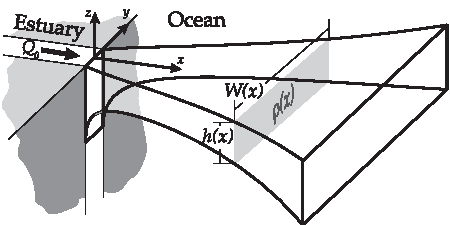
\includegraphics[width=5in]{Figures/plume_vars_flat.pdf}
    \caption{A schematic showing the variables in the simple model of a near-field plume.}
    \label{fig:plume_vars}
\end{figure}

\begin{figure}[p]
    \centering
    \includegraphics[width=4in]{Figures/plume_dilution.pdf}
    \caption{A parameter space of simulations of the simple near-field plume layer model with constant entrainment shows normalized plume dilution, $\Delta\rho \Delta\rho_0^{-1}$, as a function of normalized local entrainment, $w_e W_0^2 Q_0^{-1}$. The near-field plume does not exist, and no dilution occurs for $\Delta\rho \Delta\rho_0^{-1}$ = 1, higher dilution occurs at lower values. Parameters and value ranges include the width of the estuary mouth $Wo$ = 50 to 3000~m, the fresh water transport $Q_f$ = 10 to 3000~m$^3$~s$^{-1}$, the initial density anomaly $\Delta\rho_0$ = 1 to 24~kg~m$^{-3}$, and the entrainment velocity $w_e$ = 10$^{-4}$ to 5$\times$10$^{-3}$. The density difference between the recieving waters and fresh water is constant through the simulations, $\Delta\rho_f$ = 24~kg~m$^{-3}$.}
    \label{fig:dilution}
\end{figure}

\begin{figure}[p]
    \centering
    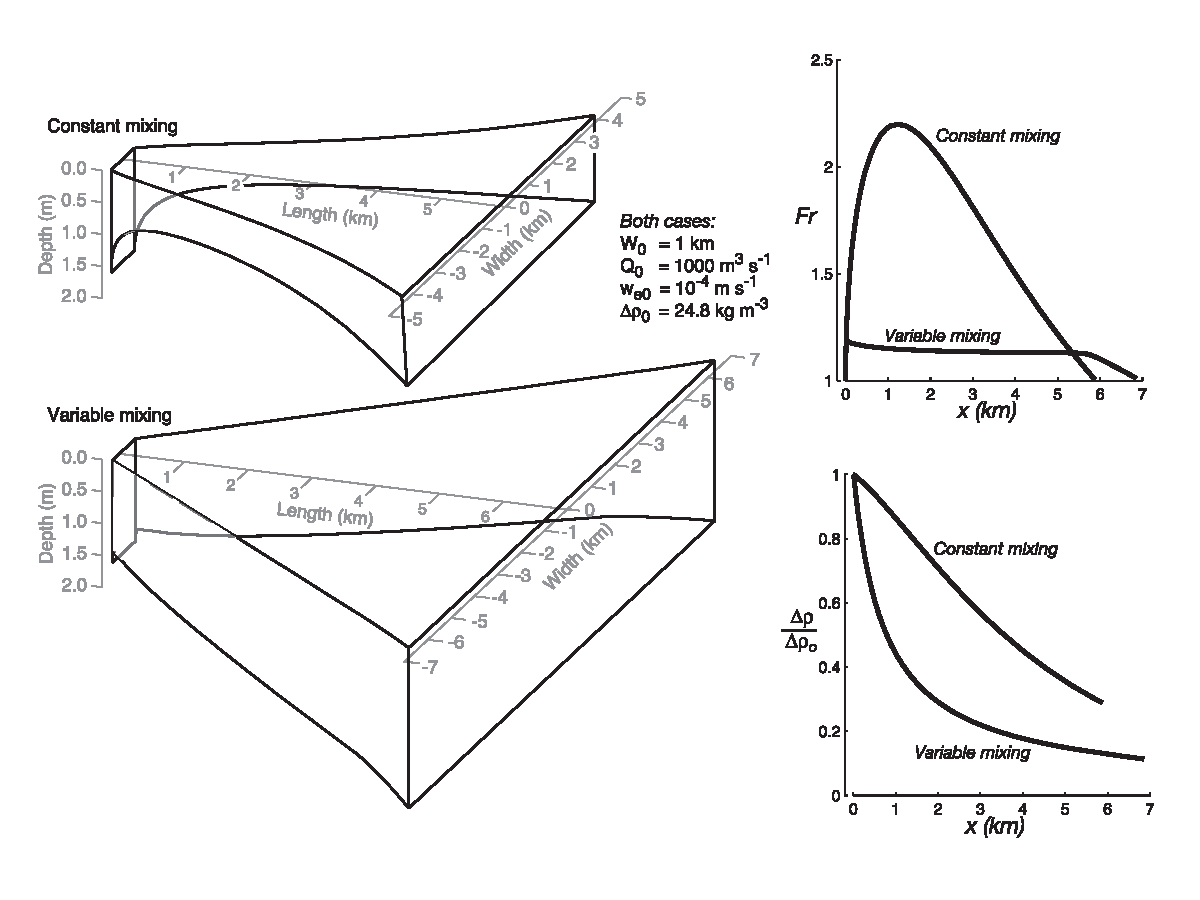
\includegraphics[width=6.5in]{Figures/plume3d_Fr_dr.pdf}
    \caption{Two idealized near-field plume simulations using constant entrainment, $w_e=w_{e0}$, and the Ellison and Turner (1959) parameterization, with a background (minimum) mixing of $w_{e0}$. The density anomaly and Froude number along the axis of each plume is shown to the right. The background mixing in the variable mixing case is triggered just before 6~km offshore, and can be seen as a kink in the Froude number profile, and in the layer thickness, but has little effect on the density anomaly. }
    \label{fig:plume3d_Fr_dr}
\end{figure}

\begin{figure}[p]
    \centering
    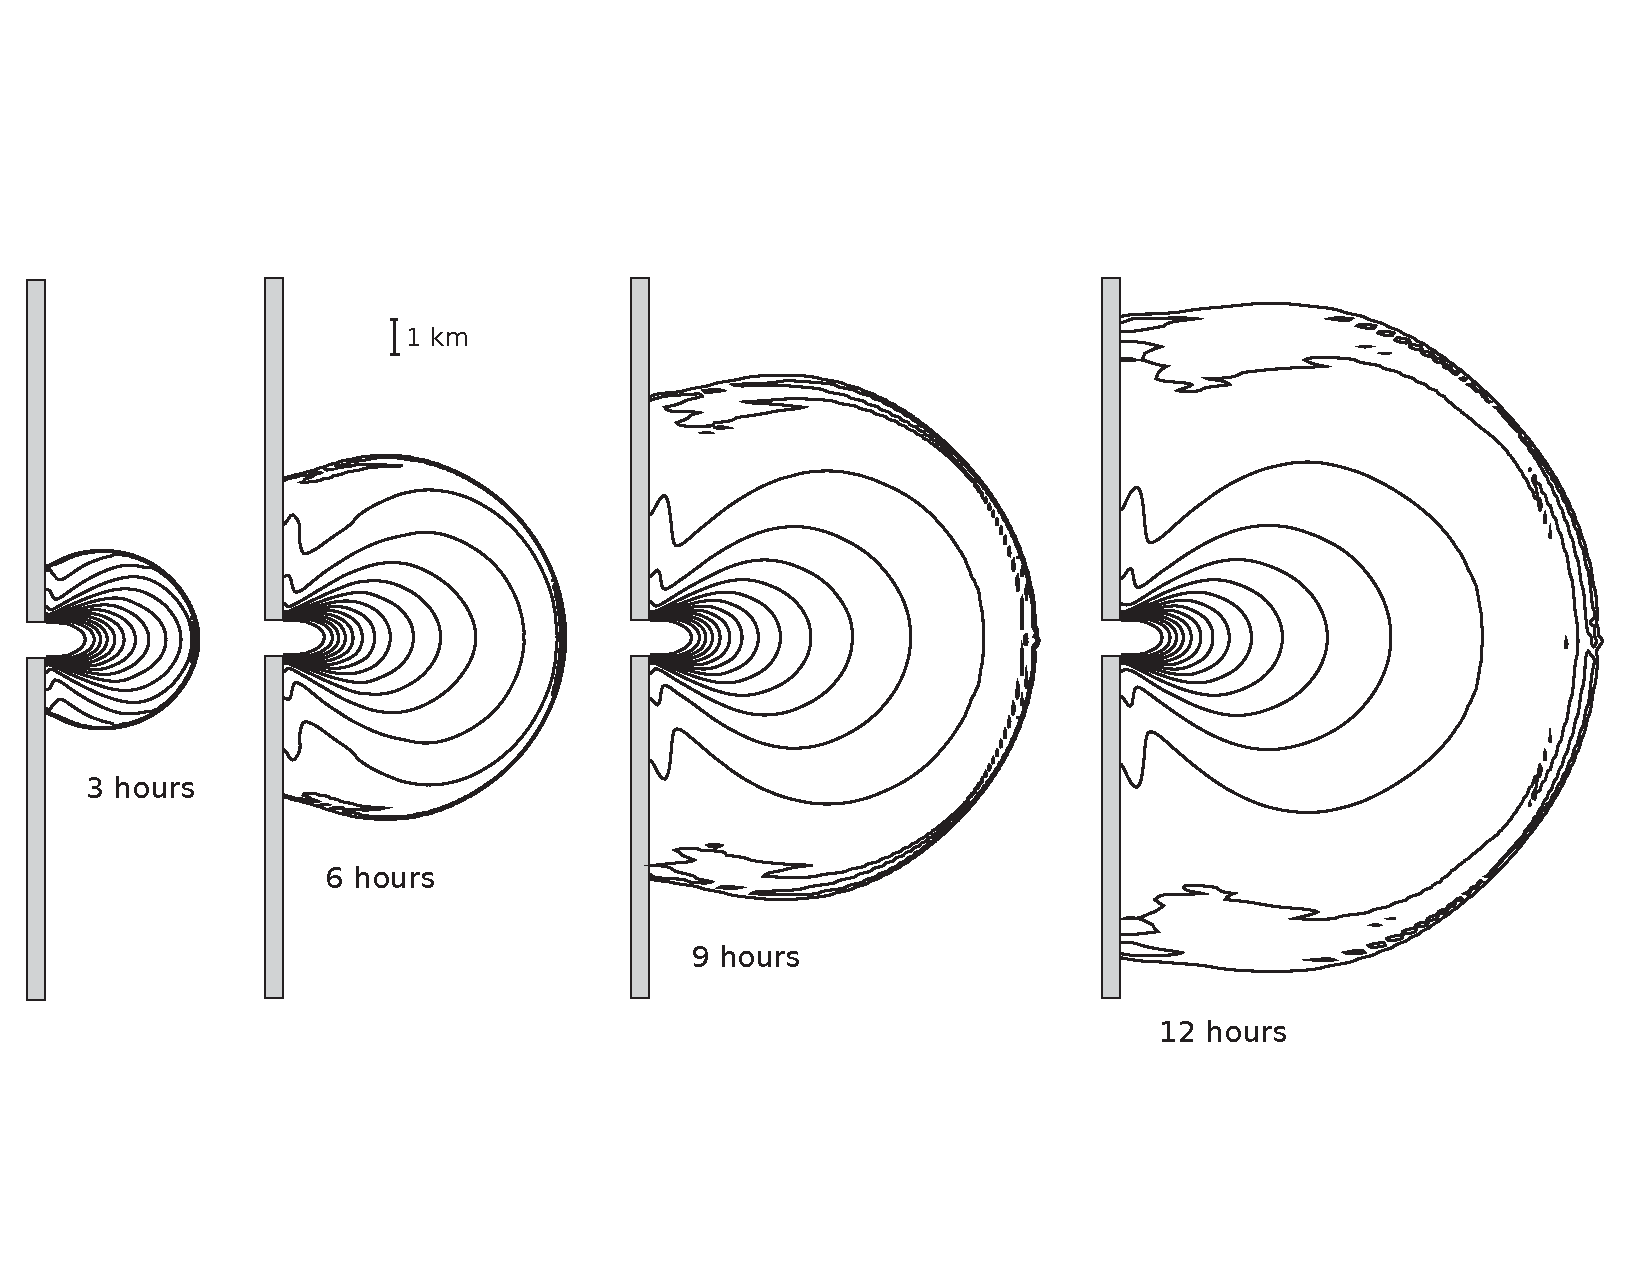
\includegraphics[width=6in]{Figures/plume_expansion_frames.pdf}
    \caption{Surface density contours are shown at four stages of plume evolution from a three-dimensional, non-linear hydrodynamic simulation using an idealized configuration.}
    \label{fig:3d_expansion}
\end{figure}


% \begin{figure}
%     \centering
%     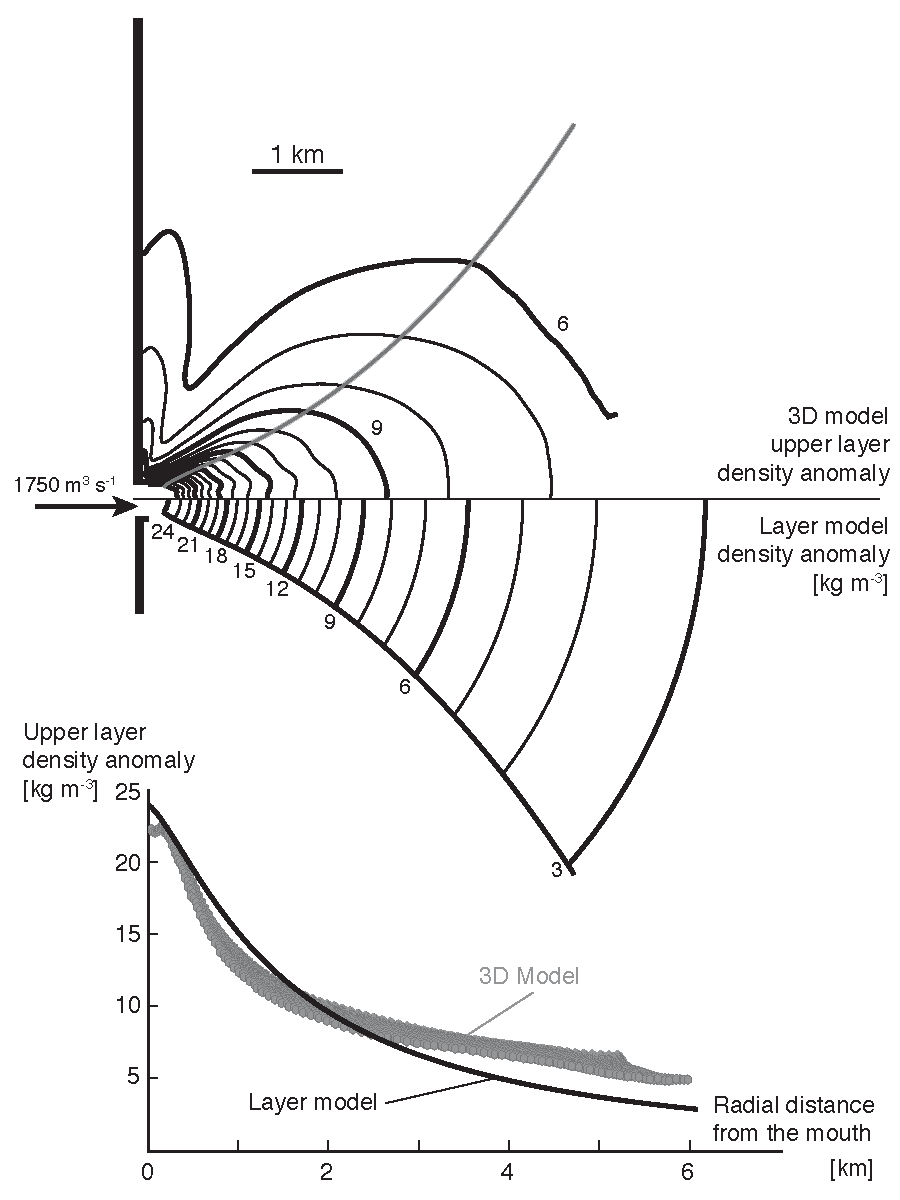
\includegraphics{Figures/ideal_comp_rev1.pdf}
%     \caption{The top panel shows an example comparing a three-dimensional, non-linear hydrodynamic simulation (top half) with a corresponding idealized layer model (bottom half). The bottom panel shows the surface layer density from both models as a function of radial distance from the mouth at the time corresponding to the snapshot shwon in the upper panel.}
%     \label{fig:mixing_comp}
% \end{figure}



\end{document}

